\documentclass[a4paper,10pt]{report}
\usepackage[utf8]{inputenc}
\usepackage[T1]{fontenc}
\usepackage[francais]{babel}
\usepackage{graphicx} 
\usepackage{enumitem}
\usepackage{underscore}
\usepackage{float}
\usepackage{array}
\usepackage{geometry}
\usepackage{titlesec} 
\usepackage{titletoc}
\usepackage{vmargin}
\usepackage{fancyhdr}

\makeatletter

\setlength{\headheight}{11.0pt}

\renewcommand{\headrulewidth}{1pt}

\titlespacing*{\chapter}
  {0pt}		% retrait à gauche
  {0pt}		% espace avant
  {30pt}	% espace après
   [0pt]	% retrait à droite
   
% Style du titre de chapitre
\titleformat{\chapter}[frame]{\huge\normalfont\sc}{\filright\footnotesize\enspace CHAPITRE \thechapter\enspace}{8pt}{\filcenter}{}
  
  
% Style de titre de section
\titleformat{\section}[hang]{\bfseries\sc}{\Large\thesection}{1em}{}


% Mise en place du Sommaire
\titlecontents{chapter}[3em]{\addvspace{1em plus 0pt}\bfseries\Large}{\contentslabel{2em}}{\hspace{-1.3em}}{\hfill\contentspage}[\addvspace{3pt}]

% Title Page
\begin{titlepage}

\title{Master 1 Bioinformatique\\Stat'n Dat}


\author{DAHMANI Amal\\JAMART Kevin\\LOPEZ Myriam\\\\}

\end{titlepage}


\begin{document}


\renewcommand{\thechapter}{\Roman{chapter}} 
\renewcommand{\thesection}{\Roman{section}}
\renewcommand{\thesubsection}{\Roman{subsection}}
\renewcommand{\contentsname}{Sommaire}
\renewcommand{\thesubsubsection}{\Roman{subsubsection}}


\maketitle
\newpage
\tableofcontents
\addtocontents{toc}{\protect\thispagestyle{empty} 
                    \protect\pagestyle{empty}}
\setcounter{tocdepth}{3}     % Dans la table des matieres
\setcounter{secnumdepth}{3}  % Avec un numero.


\newpage
\thispagestyle{empty}
\setcounter{page}{1}
\addcontentsline{toc}{section}{Introduction}

\chapter*{Introduction}


 
\chapter{Analyse et conception}


\section{Problématiques à résoudre}


\subsection{Ergonomie}

L’ergonomie logicielle est une nécessité pour l’utilisateur afin d'améliorer l'interaction homme-machine et de facilité l’utilisation du programme. Stat’n Dat se doit donc de répondre à ce besoin par l’implémentation d’une interface claire et simple. Cela permettra à l'utilisateur d’être plus rapide dans l’exécution des tâches et plus efficaces dans le choix des options à utiliser.  graphique. 

% \subsubsection{De manière générale}

% \begin{itemize}

% \item •	Permettre l'accès à des pages d'informations sur le logiciel : outil aide


% \end{itemize}


\subsubsection{Sélection de données}

La sélection des données est un partie importante du projet puisqu'elle va permettre d'axer les analyses statistiques effectuées en suivant. Pour permettre une manipulation aisée des données et leur sélection le projet nécessite certaines fonctionnalités :\\

\begin{itemize}

\item Une fenêtre permettant l'utilisation des requêtes SQL directement :\\ Suivant l'idée d'une ergonomie logicielle efficace et d'une modularité quant à l'accès aux données, notre projet doit proposer un outils permettant d'inscrire directement les requêtes SQL pour extraire de la base les données désirées.

\item Une vérification syntaxique en cas d'erreur :\\ 
L'extraction des données peut générer des erreurs. En effet, une requête SQL erronée peut, si elle n'est pas gérée, provoquer l'arrêt du impromptue du programme. C'est pourquoi il est indispensable de prévoir ces erreurs et d'implémenter un affichage clair et concis pour en informer l'utilisateur.

% \item •	Une requête "routine" : la rendre accessible facilement

\item Une visualisation claire des données sous forme de tableau :\\
Pour permettre une manipulation efficace des données, Stat'n Dat doit proposer un affichage simple du résultat de la requête envoyée. Dans ce cadre-ci un tableau reprenant l'ensemble des données extraites doit être implémenté résumant ainsi les données à traiter. 
%•	Pouvoir revenir sur son choix de sélection des données -->
\item Une modification simple de la sélection des données :\\
La requête SQL effectuée, les données extraites visualisées, il est possible que certaines valeurs ne soient pas nécessaires. C'est pourquoi Stat'n Dat doit proposer une fonctionnalité de sur-sélection des données (dans le tableau récapitulatif par exemple). Cet outil permettra d'affiner les données à traiter.

\item •	Outil de suppression de ligne de données / Tri

\item Permettre l'exception de certains sujets dits "à biais" :\\
La manipulation de données dans le cadre statistiques peut engendrer des aberrations de calculs.

\end{itemize}


\subsubsection{Analyse des données}

Stat'n Dat propose d'extraire des données d'une base SQL et d'offrir un panel de tests statistiques. Toujours de le soucis d'une ergonomie travaillée et facile d'accès l'interface proposera :\\

\begin{itemize}

\item Un accès rapide aux tests statistiques :\\
L'accès aux fonctions principales d'un logiciel est une part importante de son ergonomie. C'est pourquoi il est indispensable de proposer une identification visuelle et claire des différents tests et graphiques proposés par Stat'n Dat. 

\item La définition des tests statistiques :\\
Dans un soucis d'informer l'utilisateur efficacement, le programme devra proposer une identification claire ainsi qu'un descriptif rapide et informatif de chaque test et graphique.

% \item •	Tests paramétriques ou non --> Paramètres faciles à préciser :\\
% Dans le cadres des tests paramétriques

% \item •	Statistiques descriptives --> accès facile aux paramètres de population

% \item •	Statistiques descriptives --> accès facile aux différentes modélisations de données, de base (les graphiques)

\item La possibilité de modifier le type de représentation :\\
Les résultats des tests statistiques peuvent donner lieu à différentes représentations. Certaines permettent d'extraire plus d'informations et sont plus aisées à interpréter. C'est pourquoi Stat'n Dat devra proposer un accès facile entre les différentes représentations (courbes, nuage de points, histogrammes).

\item La levée d'exception lors du passage des paramètres des tests statistiques :\\
Les tests statistiques ont, pour la plupart, des conditions d'utilisation. En effet, certains tests statistiques nécessite un échantillon suffisamment important, ou l'application d'une loi normale sur l'échantillon (pour ne citer que ces exemples). Notre outil devra déceler s'il existes des erreurs dans les paramètres passés aux tests statistiques.

\end{itemize}

\subsection{Modularité}

Dans le cadre de notre projet un accent sera mis sur la possibilité de modifier et d'améliorer les fonctionnalités offertes par le logiciel. C'est pourquoi la modularité est un point clé du projet. L'implémentation du programme doit être conçue autour de cette notion. Le code se devra d'être clair et très lisible. Ainsi l'ajout d'autres tests statistiques sera facilité. 

La modularité comprend aussi la possibilité d'adapter le programme d'autres bases de données du système PostGreSQL.

\subsection{Rapport et synthèse}

La génération automatique d'un rapport reprenant les différents éléments (données, résultats des tests statistiques, graphiques) choisis par l'utilisateur doit être implémentée. Cette fonctionnalité fait partie des éléments essentiels propre à notre programme. L'utilisateur doit avoir la possibilité de choisir ce qui figurera dans le rapport PDF final.

Il nous semble important aussi d'implémenter la génération automatique d'un historique reprenant les différentes opérations effectuées par l'utilisateur. De la même façon il sera important de garder la trace des différentes requêtes SQL afin de créer une base de requête et facilité l'utilisation du programme.

\section{Conception du logiciel}

\subsection{Interface graphique : Présentation de la page d'accueil}

L'interface graphique aura pour but déjà de rendre l'outil plus agréable à l'utilisation, et de permettre à l'utilisateur de lancer les tâches souhaitées.\\

Cette interface sera dotée d'une barre d'outils et d’une barre de menu permettant à l'utilisateur un accès simple et rapide aux fonctions de base. \\

La barre de menu donne donc accès à :

\begin{itemize}

\item Des requêtes de base avec le bouton « Requête ».

\item Des tests statistiques et les résultats obtenus avec les différents boutons « Statistique » correspondant aux différents tests. 

\item Différents types de graphiques grâce aux boutons correspondant aux différents types de graphiques.

\item L’édition d’un rapport au format PDF des parties choisies par l'utilisateur avec le bouton « Edit ».

\end{itemize} 

La barre d’outil et ses différentes icônes, permet quant à elle de :

\begin{itemize}

\item • Créer des graphiques.

\item • Enregistrer les travaux effectués.

\item • Avoir de l'aide quant au fonctionnement de l'application.

\end{itemize}


\begin{figure}[H]

\centering
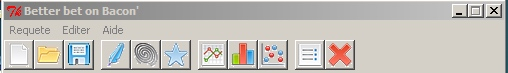
\includegraphics[scale=0.6]{barre.jpg}
\caption{Illustration de la barre d'outils}

\end{figure} 


Sur la page d’accueil, un champ libre est dédié à la réception d’une requête SQL dont nous parlerons plus loin. Un espace est également réservé à l’affichage des données.


\subsection{Connexion - Interrogation de la base de données}


En premier lieu, l'application se connectera à la base de données souhaitée. Celle-ci étant construite grâce au système PostgreSQL, le module Psycopg2 de python semble tout indiqué pour cette tâche.\\

Puis l'utilisateur disposera d'un espace dans l'interface graphique, dédié à l'insertion de la requête de son choix, celle-ci devra bien sûr être correcte ce qui demande à l’utilisateur le prérequis de la maîtrise du langage SQL.  Notre application pourra exécuter le code SQL, toujours grâce au module Psycog2.\\

La question qu’il faut se poser est comment stocker les données reçues ? Quelle structure de données allons-nous utiliser sachant qu’elle devra nous permettre de pouvoir facilement réaliser les tâches voulues à partir de ces données. Nous verrons dans la partie réalisation comment répondre à cette question.\\

Comme nous l’avons vu plus haut, il est nécessaire pour les besoins de l’utilisateur que la manipulation des requêtes soit la plus simplifiée possible, c’est pourquoi nous choisissons de mettre en place un menu déroulant « Requête » (présenté dans la partie traitant de la page d’accueil de l’IHM).\\

Pour pouvoir conserver les requêtes entre deux sessions d’exécution de Stat’nDat, nous souhaitons enregistrer ces requêtes, sous forme d’objets et les stocker dans des fichiers. C’est la raison pour laquelle nous ferons appel à une fonction de sérialisation/desérialisation pour les manipuler plus facilement. \\

Par ailleurs, le menu déroulant proposera par défaut quelques requêtes simples, de routine, qui pourront ainsi s’adapter directement à la base de données de l’utilisateur.\\

Enfin, trois boutons permettent respectivement d’effacer/annuler, valider et enregistrer la requête insérée. Cette fonction d’enregistrement de la requête est bien sûr reliée au système qui construit le menu déroulant, de manière à ce que l’on puisse retrouver sa requête directement en passant par là.


\begin{figure}[H]

\centering
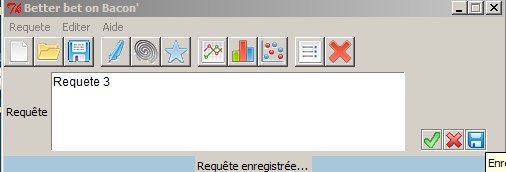
\includegraphics[scale=0.6]{requ.jpg}
\caption{Illustration de l'espace "Requête"}

\end{figure}


\subsection{Visualisation et analyse}

Les résultats seront affichés dans la deuxième partie de l'interface et dans la même fenêtre initiale, comme représenté dans la figure ci-dessous.


\begin{figure}[H]

\centering
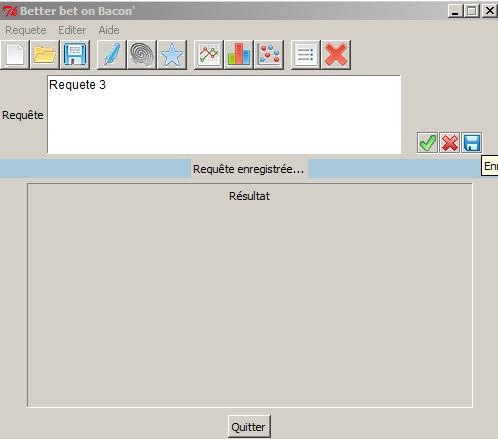
\includegraphics[scale=0.6]{res.jpg}
\caption{Illustration de l'affichage des résultats}

\end{figure}

Après affichage des résultats de la requête saisie, l'utilisateur pourra y appliquer des tests statistiques tels que les tests de Student, de Wilcoxon, ou Kruskall-Wallis. Le bilan du test effectué sera affiché dans une nouvelle fenêtre, sur laquelle sont placées des boutons correspondant aux graphiques disponibles sur l'application. L'utilisateur pourra à ce moment cliquer sur l'une des icônes pour créer un graphique qui s'affichera sur une troisième et dernière fenêtre.

\begin{figure}[H]

\centering
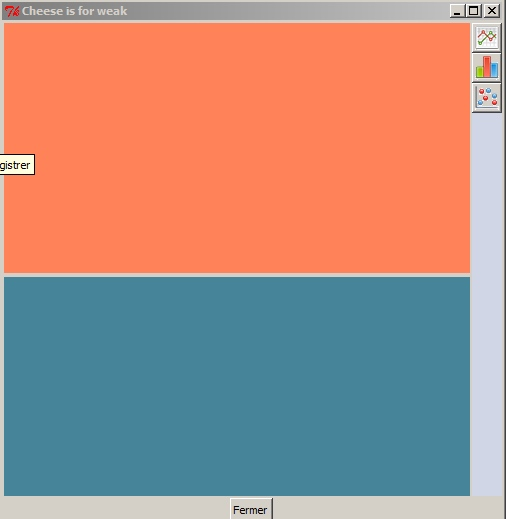
\includegraphics[scale=0.6]{test.jpg}
\caption{Illustration de l'affichage des résultats du test de Student}

\end{figure} 

L'application permet à l'utilisateur de faire une analyse  statistique des résultats obtenus des requêtes insérées. Pour effectuer les tests statistiques sur les données, l'interface graphique et les boutons décrits plus hauts permettent à l'utilisateur de lancer directement un tâche. \\

Une fois la requête lancée, le logiciel permet à l'utilisateur de visualiser ses données sous la forme d'un tableau comme décrit plus haut, c'est dans la fenêtre principale qu'un espace est spécifiquement dédié à cet usage.

La description des données, faite grâce aux différents calculs de paramètres de population est sera facultative : l'utilisateur pourra ainsi choisir s'il veut les voir apparaître ou non en fonction de ses besoins. \\
Pour cela, il lui suffira de "cocher" ou non l'option disponible dans la fenêtre de statistiques.\\

Le calcul de l'écart type, de la moyenne, et de la médiane seront faits par défaut sur tous les résultats.\\ 

L'outil donnera aussi la possibilité de créer des figures graphiques telles que les courbes, les histogrammes et les Dot-plot.\\
Des boutons permettrons à l'utilisateur de modifier directement dans la fenêtre le type de graphe. Ainsi il pourra voir successivement ses données sur plusieurs représentations différentes.\\

Grâce à Stat'nDat enfin, l'utilisateur peut générer un rapport PDF de ses résultats obtenus. L'interface lui permet de choisir la partie qui l'intéresse en ainsi générer le rapport qu'il souhaite. Pour cela, il lui suffit d'ouvrir la fenêtre dédiée à cette tâche, grâce au bouton correspondant.\\
Le rapport contiendra aussi bien les différents graphiques de représentation des données que les résultats chiffrés des tests paramétriques ou non. Enfin, et c'est le plus important, pour éviter à l'utilisateur de rédiger plusieurs fois le même "squelette" textuel, les paragraphes seront déjà présents et s'adaptent directement aux données obtenues. C'est ce qui permet l'automatisation de la tâche.


\subsection{Modifications internes}

Notre architecture logicielle comprend :

\begin{itemize}

\item • Un fichier pour gérer la partie "connexion et interrogation de la base de données".

\item • Un fichier pour gérer la partie "interface graphique".

\item • Un fichier pour gérer la partie "statistiques".

\item • Un fichier pour gérer la partie "génération du rapport PDF".

\item • Un fichier qui fera la liaison entre les quatre fichiers précédents et qui servira donc d'exécutable.

\end{itemize}


Grâce à cela, l'ajout d'un test statistique pourra se faire en passant par le code. Le module Statistique le permet, il suffit d'ajouter une fonction dans le code.
Ce simple ajout et nous nous verrons plus précisément comment dans la partie réalisation, devra suffire à ce que le test ajouté soit pris en compte dans l'interface graphique et dans la rédaction du rapport PDF.


\chapter{Réalisation}


\chapter*{Conclusion}

\addcontentsline{toc}{section}{Conclusion}

 \end{document}  